\documentclass[a4paper,11pt]{article}

\usepackage[utf8]{inputenc}
\usepackage[T1]{fontenc}
\usepackage[ngerman]{babel}
\usepackage{lmodern}
\usepackage[pdftex]{graphicx}
\usepackage{color}

\usepackage[bookmarksopen]{hyperref}
\usepackage{geometry}
 \geometry{
 a4paper,
 left=20mm,
 right=20mm,
 top=20mm,
 bottom=20mm,
 }

\parindent0em

%\usepackage{fancyhdr}
%\pagestyle{fancy}

\date{\today}
\author{Yannik Schälte}

%****************************************************************

\begin{document}

%Titelseite
\thispagestyle{empty}
\begin{center}
\vspace*{3cm}
{\Huge MiniPlaner}\\
\makebox[\linewidth]{\color{red}\rule{17.5cm}{1pt}}

\vspace*{1cm}
{\Large Handbuch}\\
\vspace*{2cm}
\begin{figure}[ht]
	\centering
  		
\includegraphics[scale=3.0]{../img/minis256.png}
	\label{fig1}
\end{figure}
\vspace*{4cm}
Yannik Schälte\\
\vspace*{5mm}
\today\\
\vspace*{5mm}
https://yannikschaelte.github.io/MiniPlaner/
\end{center}
\pagebreak

%****************************************************************

\pdfbookmark[1]{Inhaltsverzeichnis}{toc}
\tableofcontents
\thispagestyle{empty}

%****************************************************************

\section*{Übersicht}
\addcontentsline{toc}{section}{Übersicht}
Das Programm \texttt{MiniPlaner} ist ein Werkzeug zur effizienten Erstellung hochwertiger Messdienerpläne. Es ist sehr übersichtlich gehalten, bietet jedoch vielfältige Einstellungsmöglichkeiten: Messdiener und Termine können auf verschiedene Weisen gruppiert werden, das flexible Dienst-System lässt individuelle Maßlösungen zu. Nach der Eingabe aller benötigten Daten können schnell Pläne erstellt werden, interaktiv oder automatisch mittels eines Algorithmus, welcher verschiedene einen gelungenen Plan ausmachenden Faktoren gleichzeitig zu berücksichtigen versucht. Der Export der graphisch aufbereiteten fertigen Pläne ist in verschiedenen Formaten möglich -- als Webseite oder im Tabellenformat zum Ausdrucken.
%****************************************************************
\section{Installation}
Vorausgesetzt bei dieser Installation ist das Betriebssystem Windows XP oder höher (32/64 bit).
Die Installation ist sehr einfach: Entpacken Sie die erhaltene ZIP- oder 7Z-Datei (Rechtsklick + Extrahieren), oder folgen Sie den Anweisungen des Installers \texttt{MiniPlaner\_Setup}. In jedem Fall erhalten Sie ein Verzeichnis \texttt{MiniPlaner/}, in welchem diverse Unterordner sowie die ausführbare Datei \texttt{MiniPlaner.exe} enthalten sind. Dabei handelt es sich um das Hauptprogramm, welches durch einen Doppelklick gestartet werden kann. Verwenden Sie den Installer, erhalten Sie zusätzlich auf Wunsch einen Desktop-Shortcut. Eine Deinstallation kann ebenso einfach erfolgen, indem das Verzeichnis \texttt{MiniPlaner/} wieder gelöscht wird (und ggf. der Desktop-Shortcut). Das Programm schreibt lediglich in dieses Verzeichnis Daten.
\begin{figure}[ht]
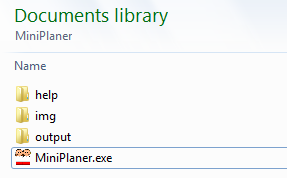
\includegraphics[scale=0.7]{filesystem.PNG}
\end{figure}
%****************************************************************
\pagebreak
\section{Dateneingabe}
Nach Programmstart gelangen Sie unmittelbar auf die zentrale Übersichtsseite der Dateneingabe.
\begin{figure}[h]
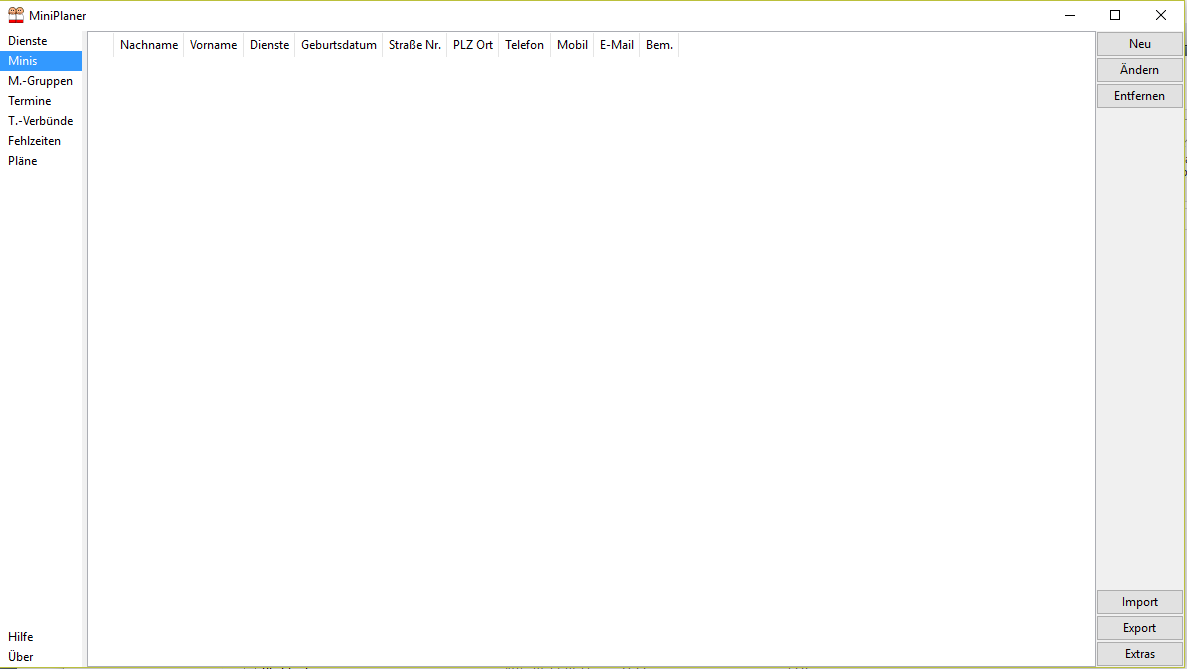
\includegraphics[scale=0.4]{hauptfenster2.PNG}
\end{figure}

Auf der linken Seite befindet sich die Navigation mit den 7 Daten-Kategorien sowie 2 Informationsseiten. Sämtliche Seiten ähneln der zum Start geöffneten Ministranten-Ansicht: In der Mitte des Fensters werden die Daten in einer Listenansicht dargestellt. Nach Selektieren einer Zeile haben Sie die Möglichkeit, diese über die Knöpfe in der rechten oberen Ecke zu löschen oder zu ändern. Genau wie das Erstellen neuer Daten geschieht dies über eine Eingabemaske.\\
Durch Klicken auf \texttt{Neu} auf der rechten Seite des Reiters \texttt{Dienste} erscheint ein Dialog, in welchem Sie dem Dienst einen eindeutigen Namen zuweisen können.
\begin{figure}[h]
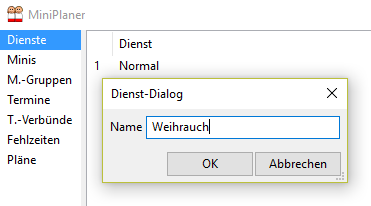
\includegraphics[scale=0.6]{dienste2.PNG}
\end{figure}
Nach Bestätigung durch \texttt{OK} erscheint der neue Dienst alphabetisch einsortiert in der Liste. Über \texttt{Ändern} kann der Name geändert werden, über \texttt{Entfernen} kann der Dienst wieder entfernt werden (Abkürzungen: Doppelklick bzw. Entf). Bei den weiteren Kategorien mit Ausnahme der Pläne ist die Vorgehensweise entsprechend. Bei den Diensten ist zu Beginn ein Standard-Dienst \textit{Normal} vorhanden, der ebenfalls modifiziert werden kann.\\
\\
\textbf{Achtung:} \textit{Entfernen} Sie eine Dateneinheit, so werden sämtliche Referenzen darauf, die eventuell von anderen Daten gemacht wurden (wie die Zuordnung von Diensten zu Terminen), ebenfalls gelöscht. \textit{Ändern} Sie lediglich Eigenschaften einer Dateneinheit, so werden Referenzen auf dieses Objekt angepasst, nicht gelöscht. Dies betrifft nicht bereits erstellte Plan-Dialoge, deren Daten nur einmal eingelesen werden. \\
\\
Es empfiehlt sich, die 7 Kategorien mehr oder weniger von oben nach unten abzuarbeiten, beginnend bei der Eingabe benötigter Dienste:
%****************************************************************
\subsection{Dienste}
Ein \texttt{Dienst} beschreibt eine Tätigkeit in der Messe (normale Ministrantentätigkeit, Weihrauch etc.). Ein Ministrant kann zu bestimmten Diensten befähigt sein, zu einem Termin werden jeweils Anzahlen von Ministranten für verschiedene Dienste benötigt. \texttt{Name} ist die Bezeichnung des Dienstes und muss eindeutig sein.\\
Über die flexible Erstellung von Diensten haben Sie einigen Individualisierungsspielraum. So können Sie auch Lektoren oder Priester verwalten oder einen Dienst \textit{Senior} kreieren, so dass alle Ministranten den Dienst \textit{Normal} ausüben können, ältere zusätzlich aber auch diesen Dienst. Müssen Sie etwa 4 Ministranten einteilen, so können Sie dann 3 Normale und 1 Senior fordern, um sicherzugehen, dass mindestens ein erfahrenerer Ministrant dabei ist. Die Dienstbezeichnungen müssen im späteren Plan nicht notwendigerweise angezeigt werden.
%****************************************************************
\subsection{Minis}
Ein \texttt{Mini(strant)} muss eindeutig über \texttt{Nachname} und \texttt{Vorname} identifizierbar sein, da er damit im Plan erscheint. Dies sind die einzigen benötigten Felder.
\begin{figure}[h]
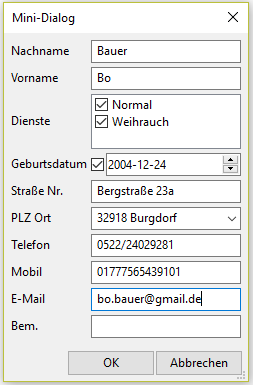
\includegraphics[scale=0.7]{messdiener2.PNG}
\end{figure}
Im Feld \texttt{Dienste} kann ausgewählt werden, zu welchen Diensten der Messdiener befähigt ist. Das \texttt{Geburtsdatum} wird nur eingelesen, wenn der dazugehörige Haken aktiviert ist. Das Feld \texttt{Bem.} kann für beliebige Anmerkungen genutzt werden. Die restlichen Felder sind selbsterklärend.\\
Eine Besonderheit beim Reiter \texttt{Mini} ist, dass es auf der rechten Seite unten 2 zusätzliche Knöpfe gibt. Falls bereits eine Messdienerliste in einem Tabellenformat vorliegt, so kann der \texttt{Import} dieser den zeitlichen Aufwand des Einstellens der Daten ungemein verringern. Dazu muss jene Datei ggf. umsortiert und in ein einfaches CSV-Format umgewandelt werden (die gängigen Tabellenkalkulationsprogramme bieten diesen Service), so dass sie eingelesen werden kann.
\begin{figure}[h!]
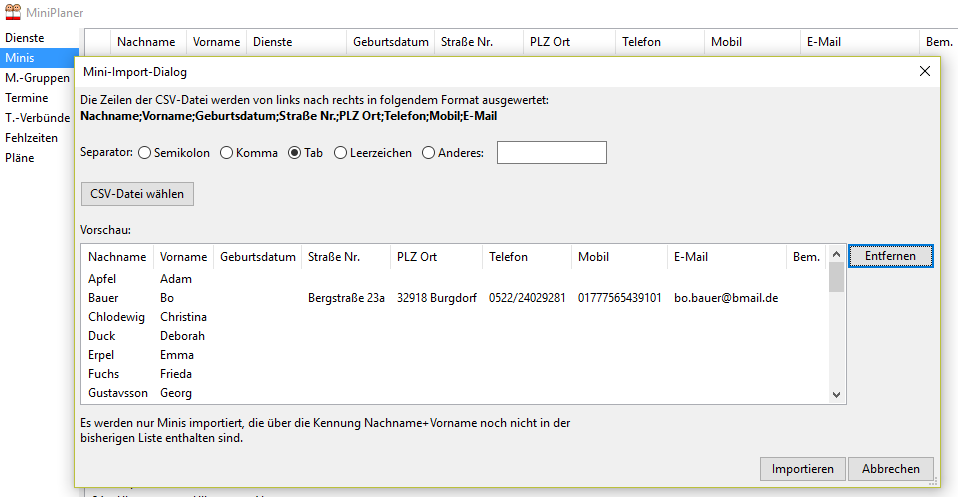
\includegraphics[scale=0.50]{mini_import2.PNG}
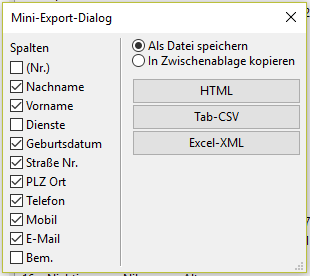
\includegraphics[scale=0.50]{mini_export2.PNG}
\end{figure}

Der Knopf \texttt{Export} bietet die Möglichkeit, die Messdienerliste in verschiedene Formate zu exportieren. Die einzelnen Formate werden im Abschnitt zum Export von Plänen näher dargestellt.

Der Knopf \texttt{Extras} erlaubt es schließlich, automatisiert eine Liste aller verfügbaren (E-Mail-)Adressen zu erstellen und in die Zwischenablage zu kopieren, wobei fehlende Adressen direkt angezeigt werden, damit mit diesen anderweitig verfahren werden kann.
%****************************************************************
\subsection{M.-Gruppen}
Oft hat man Meinistranten, etwa Geschwister, die gern zusammen aufgestellt werden möchten. Dies ist in der Kategorie \texttt{M.-Gruppen} (i.e.\ Ministranten-Gruppen) in 2 Varianten möglich: 
\begin{figure}[h!]
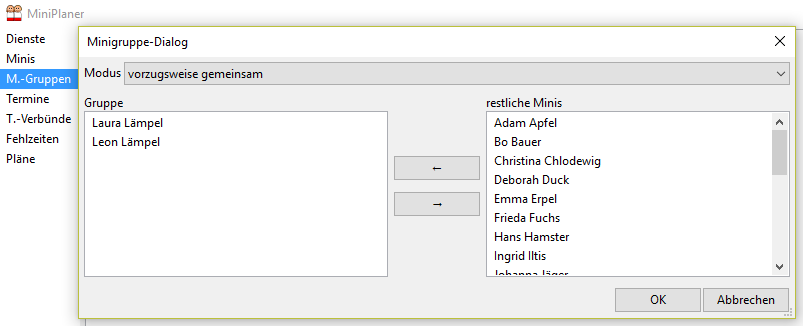
\includegraphics[scale=0.6]{mgruppe2.PNG}
\end{figure}

Im Modus \texttt{vorzugsweise gemeinsam} werden die Gruppenmitglieder nach Möglichkeit an einem Termin (ggf. in verschiedenen Diensten) gemeinsam aufgestellt, allerdings eventuell nicht immer. Im Modus \texttt{ausschließlich gemeinsam} werden an einem Termin entweder sämtliche Gruppenmitglieder aufgestellt oder keines. Ist etwa ein Mitglied verhindert, so wird die ganze Gruppe nicht aufgestellt.
%****************************************************************
\subsection{Termine}
Ein \texttt{Termin} beschreibt z.B. einen Gottesdienst, zu welchem Ministranten benötigt werden. Im Reiter \texttt{Termine} werden die Termine zur besseren Übersicht in 2 separaten Listen verwaltet: Neben den einmaligen \texttt{Einzelterminen} gibt es zum Verwalten periodisch wiederkehrender Termine die \texttt{Serientermine}.
\begin{figure}[h]
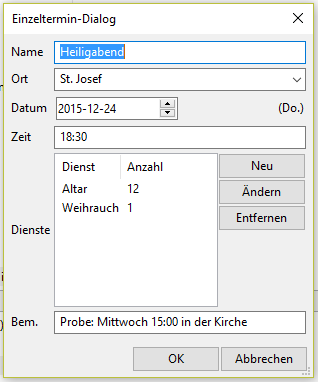
\includegraphics[scale=0.55]{einzel2.PNG}
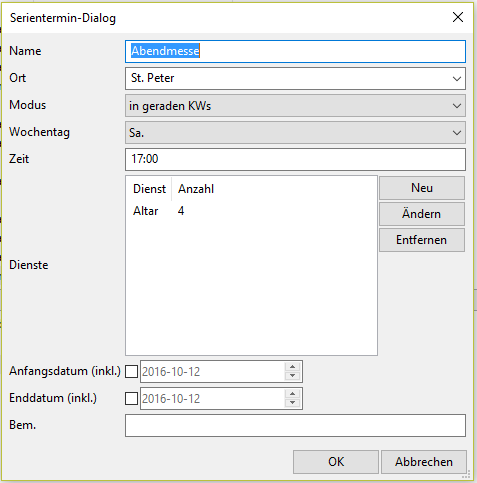
\includegraphics[scale=0.55]{serie2.PNG}
\end{figure}

\texttt{Einzeltermine:} Obligatorische Angaben sind das \texttt{Datum}, die \texttt{Zeit} und die benötigten \texttt{Dienste}. Name, Ort und Bemerkung werden im Plan nur angezeigt, wenn die entsprechenden Felder gefüllt sind. Über den Knopf \texttt{Import} haben Sie zusätzlich die Möglichkeit, direkt eine in einem CSV-Format vorliegende Liste von einzelnen Terminen zu importieren. Beachten Sie jedoch, dass bei einem Import nicht alle Möglichkeiten des Programms unmittelbar genutzt werden können (z.B.\, verschiedene Dienste, T.-Gruppen). Verwenden Sie ggf. lieber Serientermine.\\
\texttt{Serientermine:} Diese eignen sich hervorragend zur Verwaltung regelmäßig wiederkehrender Termine. Unter \texttt{Modus} kann man verschiedene selbsterklärende Periodenarten auswählen, es erscheinen entsprechende Felder. Optional kann man zusätzlich Anfangs- und Enddatum angeben, zwischen denen der Termin auftritt. Wird eines der beiden Felder freigelassen (d.h. der Haken nicht gesetzt), so gibt es zeitlich nach unten bzw. nach oben keine Schranke.
%****************************************************************
\subsection{T.-Verbünde}
In einem \texttt{T.-Verbund} (i.e.\ Termin-Verbund) können Termine zusammengefasst werden, die inhaltlich zusammengehören, etwa weil die gleiche Messe gelesen wird. Jeder Ministrant kann dann im gesamten Termin-Verbund höchstens einmal eingesetzt werden. Ist im Verbund mindestens ein Termin ein Serientermin, so werden die Termine wöchentlich zusammengefasst: Jeweils nach dem dann einzugebenden Start-Wochentag werden alle Termine, die in den nächsten 7 Tagen anfallen, zu einem Termin-Verbund gruppiert. Termine in der darauffolgenden Woche bilden einen eigenen Verbund.
\begin{figure}[ht]
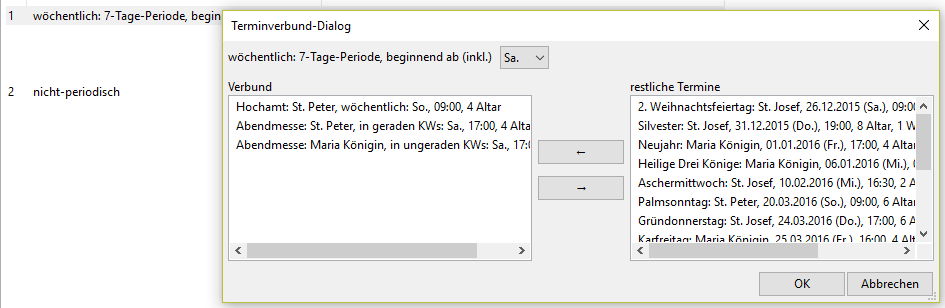
\includegraphics[scale=0.6]{tgruppe2.PNG}
\end{figure}
%****************************************************************
\subsection{Fehlzeiten}
Es gibt 3 Möglichkeiten, für einen Ministrant eine \texttt{Fehlzeit} zu erstellen, während welcher er nicht eingeteilt werden kann:
\begin{figure}[ht]
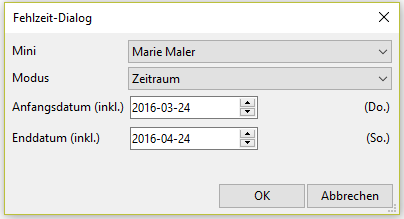
\includegraphics[scale=0.6]{fehlzeit2.PNG}
\end{figure}

Es kann ein zusammenhängender Zeitraum oder ein Wochentag mit Zeitfenster eingegeben werden, oder es kann ein Termin benannt werden, zu welchem der Messdiener unpässlich ist.
%****************************************************************
\subsection{Pläne}
Nachdem alle benötigten Daten eingegeben worden sind, kann ein neuer Plan erstellt werden. Nach einem Klick auf \texttt{Neu} im Reiter \texttt{Pläne} ist zunächst der Zeitraum anzugeben. Bei einem Klick auf \texttt{Weiter} werden einmalig sämtliche benötigten Daten eingelesen und anhand der eingestellten Einzel- und Serientermine alle in diesem Zeitraum anfallenden Termine berechnet. Spätere Änderungen an den Daten im Hauptfenster haben also keinen Einfluss mehr auf diesen Plan. 

Nun haben Sie noch einmal die Möglichkeit, Veränderungen an den Termindaten vorzunehmen und zu schauen, ob Sie die Termin-Verbünde richtig eingegeben haben. Klicken Sie anschließend auf \texttt{Weiter}, erscheint eine zentrale Übersichtsseite, in welcher alle Aktionen zum Füllen und Exportieren des Planes zusammengestellt sind.
\begin{figure}[ht]
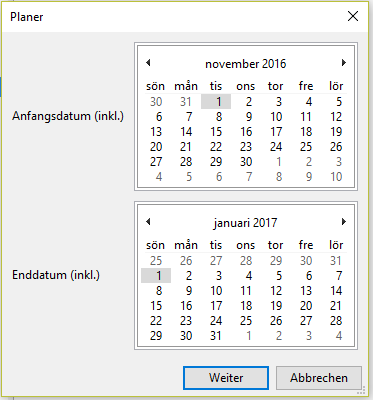
\includegraphics[scale=0.52]{planer_zeitraum2.PNG}
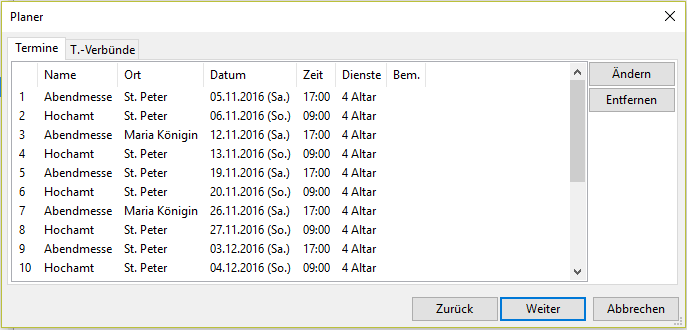
\includegraphics[scale=0.52]{planer_termine2.PNG}
\end{figure}

\pagebreak

Eine Besonderheit im Reiter \texttt{Pläne} ist, dass über den Knopf \texttt{Extras} im daraufhin erscheinenden \texttt{MiniInterface-Dialog} die Möglichkeit besteht, ein Web-Formular zu erstellen (im Reiter \texttt{Daten für MiniInterface-Formular exportieren}), das auf die Homepage der Gemeinde gestellt werden kann. Über dieses Interface können die Messdiener von Zuhause über einen Browser selbst eintragen, wann sie dienen können oder nicht können. Diese Daten können dann direkt automatisiert in das Programm eingelesen werden (über den Reiter \texttt{Mit Daten aus MiniInterface-Formular Plan erstellen}) und wie üblich anschließend per Knopfdruck die restlichen Einsätze zufällig verteilt und der Plan ausgedruckt werden. Über dieses Add-On wird also eine einfache und schnelle Interaktion mit den Messdienern bei der Plan-Erstellung ermöglicht, es muss freilich aber nicht benutzt werden.\\
Die hierzu benötigte Datei \texttt{MiniInterface.php} finden Sie auf der Projekthomepage. Diese Datei packen Sie einmalig auf den Server und wenn Sie einen Plan erstellen wollen, packen Sie in das gleiche Verzeichnis die Datei \texttt{MiniInterface.dat}, die in der oben genannten Ansicht erstellt werden kann. Beachten Sie, dass Sie selbst für die Sicherheit der Daten auf dem Server Sorge tragen müssen (z.B. durch Passwortschutz). \\
Zu den Details dieses Add-Ons dürfen Sie mich gern noch mal fragen.
\begin{figure}[ht]
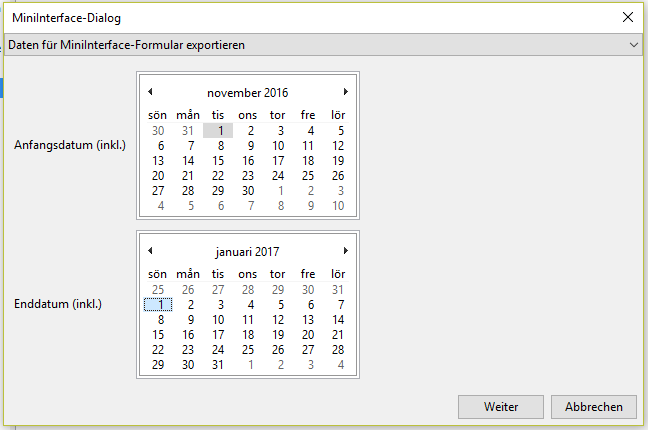
\includegraphics[scale=0.6]{miniinterfacedialog2.PNG}
\end{figure}
%****************************************************************
\pagebreak

\section{Planerstellung}
Auf der linken Seite des Planer-Fensters finden sich zur Information die wichtigsten Daten zu Ministranten, Ministranten-Gruppen und Termin-Verbünden. Bei den Ministranten können Sie im Feld \texttt{Einsätze} vergleichen, wer wie oft eingesetzt wurde.\\
Auf der rechten Seite finden sich Knöpfe zum Bearbeiten der Daten des Planes sowie zum Export: Über \texttt{Automatisch} starten Sie den Algorithmus zur Berechnung einer möglichen Lösung des Planes, Parameter dazu können Sie über \texttt{Einstellungen} eingeben. Dauert die Lösung eines Planes etwas länger, kann über \texttt{Stoppen} der Vorgang abgebrochen werden. Neben zwei Vor- und Zurück-Tasten können Sie über \texttt{Leeren} die Einträge des Planes komplett löschen. Über \texttt{Speichern} können Sie den aktuellen Zustand des Planes sichern.
\begin{figure}[h]
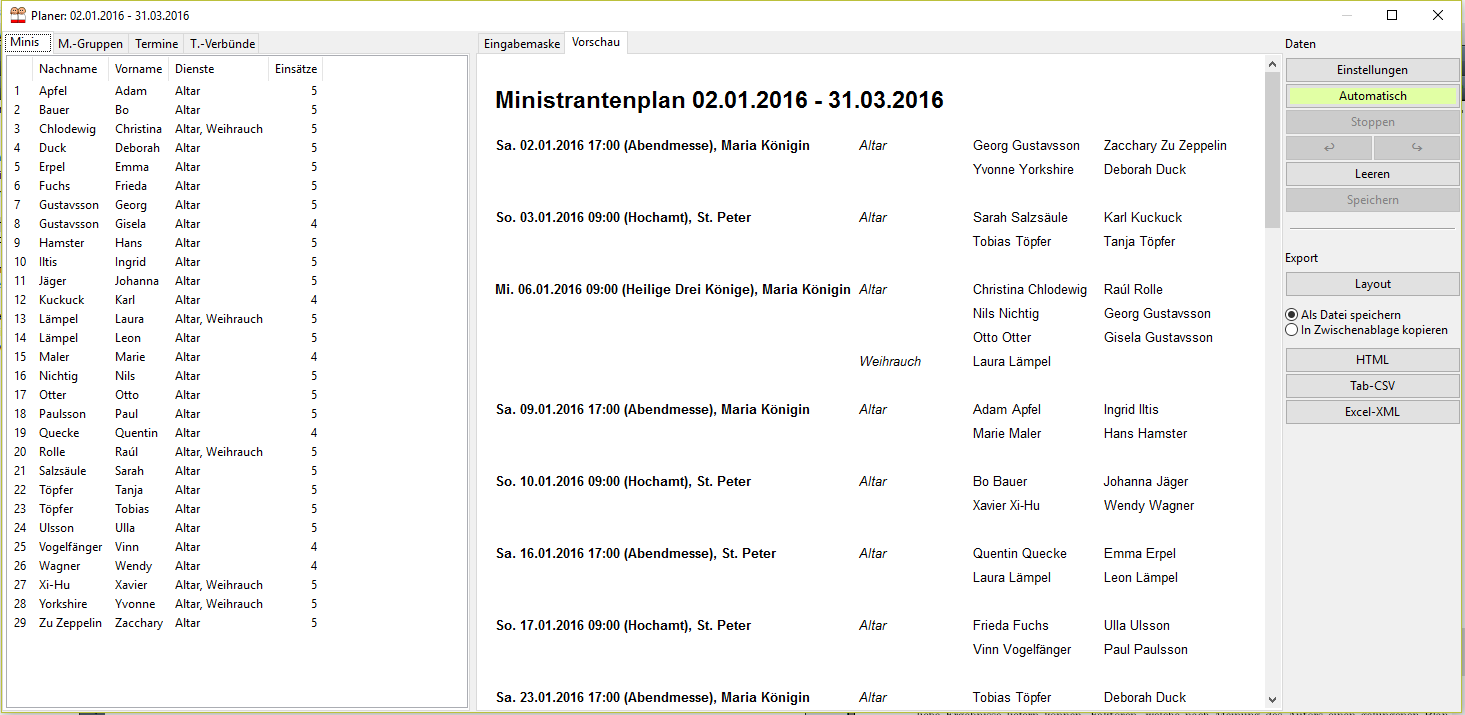
\includegraphics[scale=0.4]{planer2.PNG}
\end{figure}

Im mittleren Bereich finden sich zwei Ansichten des Planes: Eine HTML-\texttt{Vorschau} sowie eine interaktive \texttt{Eingabemaske}, welche zum erstmaligen Laden eine gewisse Zeit benötigt. In der Vorschau können Sie das Layout des Planes, das Sie über den Knopf \texttt{Layout} variieren, begutachten. In der Eingabemaske haben Sie die Option, selbst Messdiener zuzuweisen. Dies wird in den folgenden Abschnitten näher erläutert.

%****************************************************************
\subsection{Automatisch}
Über die Algorithmus-\texttt{Einstellungen} haben Sie die Möglichkeit, festzulegen, dass längere Fehlzeiträume eines Messdieners gemäß Einsatz-Wahrscheinlichkeit anteilig angerechnet werden, d.h. der Messdiener wird insgesamt etwas weniger eingesetzt. Dies betrifft lediglich Fehlzeiten vom Typ \texttt{Zeitraum}, nicht aber wöchentliche Fehlzeiten oder Unpässlichkeit bei bestimmten Terminen. Wird diese Option nicht gewählt, so wird versucht, auch diesen Messdiener etwa gleich oft wie die anderen einzusetzen.\\
Beim Algorithmus selbst haben Sie 2 Varianten zur Auswahl, die je nach Situation leicht unterschiedliche Ergebnisse liefern können. Faktoren, welche nach Meinung des Autors einen gelungenen Plan ausmachen und die hier berücksichtigt und im Zusammenspiel gewichtet werden, sind:
\begin{itemize}
\item Jeder Messdiener sollte in etwa gleich oft eingeteilt werden. Dabei gibt es natürlich Unterschiede, wenn die Messdiener unterschiedliche Fähigkeiten haben, die unterschiedlich oft benötigt werden.
\item Die Verteilung der Einsätze eines Messdieners über den Zeitraum des Planes sollte einigermaßen gleichmäßig sein.
\item Andererseits sollte der Plan zu einem gewissen Grad zufällig sein, so dass die Konstellationen abwechslungsreich sind, sich nicht immer die gleichen Paare bilden.
\item Die Bedingungen an Ministranten-Gruppen und Termin-Verbünde müssen beachtet werden.
\end{itemize}
Um Ihnen bei der interaktiven Planung weitergehende Freiheiten zu geben, werden die Ministranten-Gruppen erst bei Start des Berechnungsvorgangs nach Klick auf \texttt{Automatisch} ausgewertet, manuell haben Sie die Möglichkeit, von diesen abzuweichen. Schon vorher fest eingeplant werden Termin-Verbünde, Fähigkeiten und eingetragene Fehlzeiten.\\
Auf die Möglichkeit, festzustellen, ob ein Plan überhaupt eine Lösung besitzt, wurde verzichtet, weil ein solcher Vorgang entweder nur triviale Lösungen liefert, die nicht zu gebrauchen sind, weil oben genannte Faktoren unzureichend beachtet werden, oder er kommt dem zufallbehafteten Algorithmus unter \texttt{Automatisch} sehr nahe. Klicken Sie auf diesen Knopf, werden allerdings einige grundlegende Überprüfungen angestellt und es wird eine Fehlermeldung ausgegeben, wenn der Plan als unlösbar erkannt wurde. Sollte das Programm doch einmal länger benötigen (mehrere Sekunden), so ist es wahrscheinlich, dass sich keine Lösung finden lässt. Dann beenden Sie den Prozess über \texttt{Stoppen} und kehren zur Hauptseite zurück, um die Vorgaben, an denen es scheitern könnte, flexibler zu gestalten. Anschließend starten Sie einen neuen Planer. Es mag sinnvoll sein, die Vorgaben von vornherein zunächst nicht zu fest anzusetzen.
%****************************************************************
\subsection{Interaktiv}
Öffnen Sie den Reiter \texttt{Eingabemaske}, so haben Sie die Option, neben der automatischen Berechnung des Planes individuelle Anpassungen vorzunehmen. Klicken Sie doppelt auf ein umrandetes Feld, so können Sie diesem einen Messdiener aus einer Vorschlagsliste aller an diesem Termin (noch) verfügbaren Messdiener zuweisen. So können Sie das Programm auch als einfache Eingabehilfe benutzen und alle Eintragungen selbst vornehmen. Klicken Sie einfach auf ein gefülltes Feld oder auf eine Zeile in der Messdienerliste links, so können sie graphisch die Einsätze dieses Messdieners im gesamten Planungszeitraum nachvollziehen.
\begin{figure}[h]
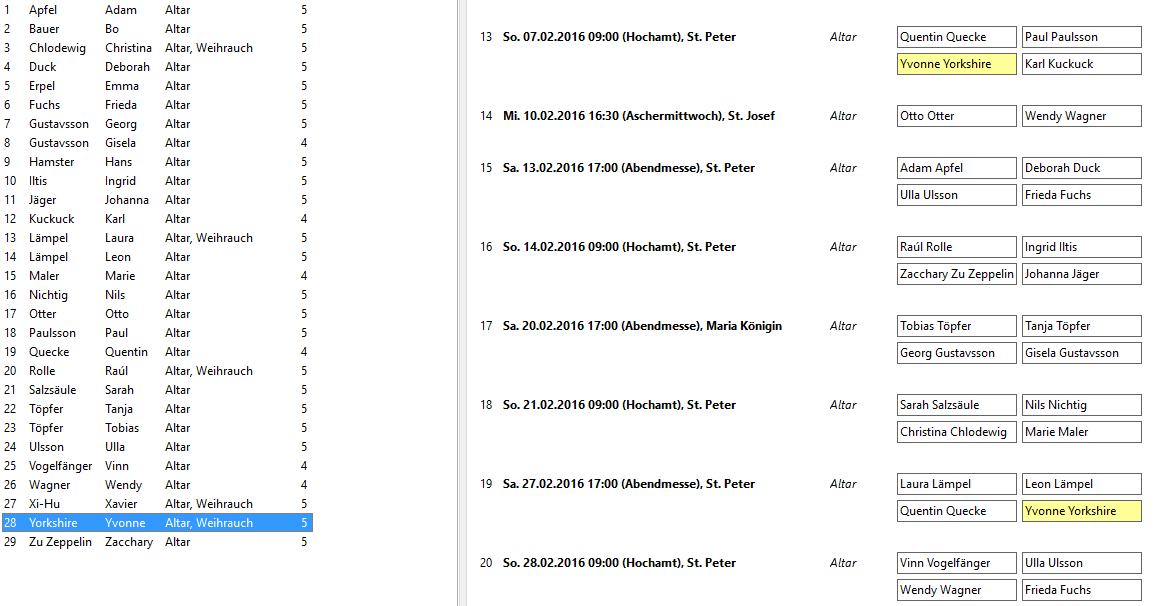
\includegraphics[scale=0.4]{highlight2.PNG}
\end{figure}
%****************************************************************
\subsection{Export}
Der Export wird auf 2 Wegen ermöglicht: Durch Speichern als Datei oder kopieren in die Zwischenablage, so dass Sie den Code (per Strg + V bzw. Rechtsklick + Einfügen) in ein Darstellungsprogramm einfügen können.\\
Es werden 3 verschiedene Formate angeboten: \texttt{CSV}-Dateien mit dem Tabulator-Zeichen als Separator können von allen gängigen Tabellenkalkulationsprogrammen gelesen werden, besitzen allerdings keine Stil-Informationen. Dateien im Format \texttt{Excel-XML} können problemlos mit dem Programm \texttt{Microsoft Excel} geöffnet werden, aber auch mit anderen Programmen wie \texttt{LibreOffice} und \texttt{OpenOffice}. Hinweise von \texttt{Excel}, dass Kompatibilitätsprobleme auftreten können, sind ggf. zu ignorieren. In diesen Programmen können Sie dann abschließende Änderungen vornehmen, Text hinzufügen und den Plan ausdrucken.\\ 
Eine weitere Variante, bei welcher wie im XML-Format Stil-Informationen erhalten bleiben, ist der Export als \texttt{HTML}-Datei, welche in einem beliebigen Browser wie \texttt{Firefox} oder \texttt{Chrome} angezeigt und so auch in eine Webseite eingebunden werden kann. Wenn Sie sich ein wenig mit HTML und CSS auskennen, können Sie die Darstellungsparameter des Dokumentes wie Hintergrundfarben und Textart praktisch mittels weniger CSS-Styles am Kopf der HTML-Datei individualisieren. Sie können allerdings auch den HTML-Code (oder den CSV-Code) in die Zwischenablage kopieren und per Strg + V in ein geöffnetes \texttt{Excel}-Dokument einfügen. Sämtliche dieser Varianten haben sich als praktikabel erwiesen.\\
Überall im Programm, so auch für die Export-Dateien, wird die Unicode-Kodierung UTF-8 verwendet.
\begin{figure}[h]
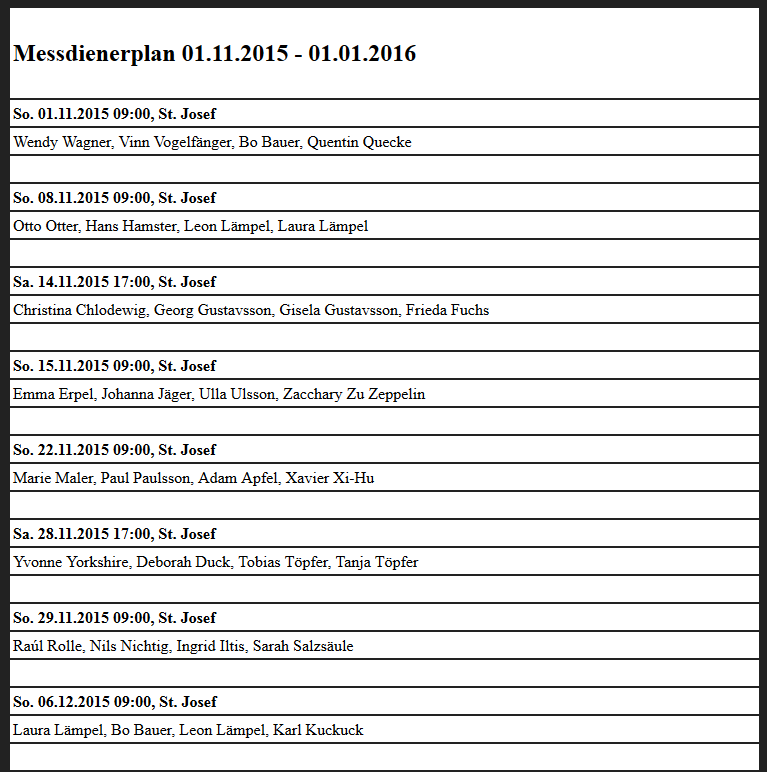
\includegraphics[scale=0.3]{html1.PNG}
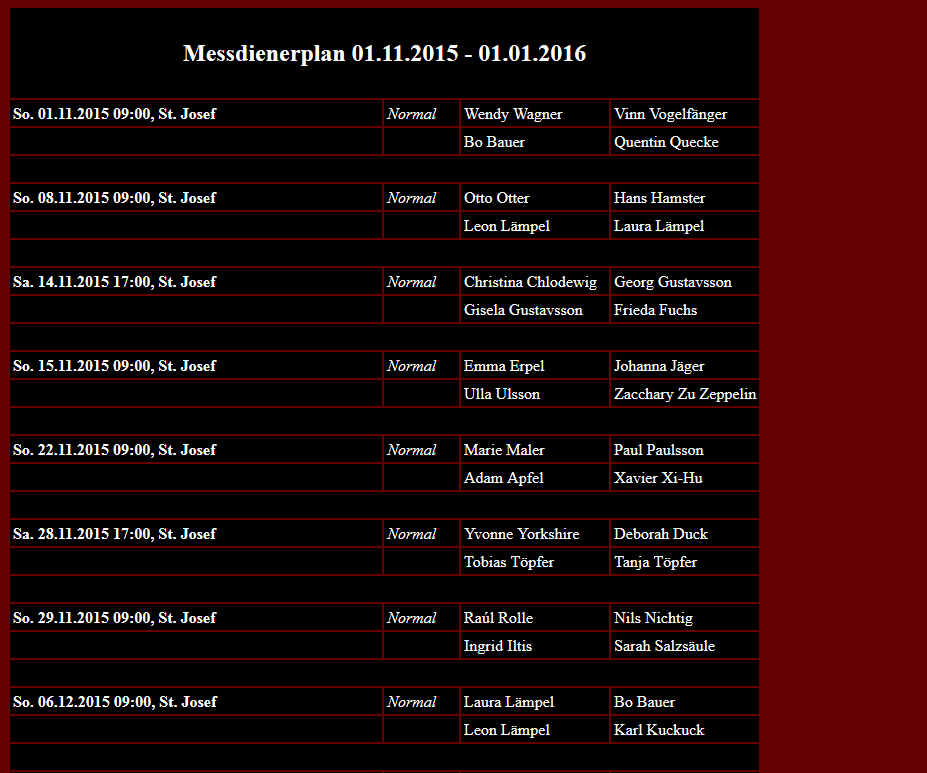
\includegraphics[scale=0.3]{html2.PNG}
\end{figure}
\section*{Autorennotiz}
\addcontentsline{toc}{section}{Autorennotiz}
Das vorliegende Programm wurde im Praxis-Einsatz und in vielen verschiedenen Szenarien getestet. Dennoch ist es sicherlich nicht möglich, allen Anforderungen gerecht zu werden. Für etwaige Enttäuschungen und Frustration bitte ich im Voraus um Verzeihung. Über Rückmeldungen (z.B. an yannik.schaelte@gmail.com) würde ich mich sehr freuen, um das Programm verbessern zu können. Bei Fragen, Programmfehlern, Problemen oder Ideen dürfen Sie sich gern jederzeit bei mir melden. Ich hoffe, der \texttt{MiniPlaner} ist Ihnen bei Ihrer Arbeit hilfreich.
\vspace*{2cm}

Bielefeld, \today\\
Yannik Schälte
\end{document}